%#Split: 01_background  
%#PieceName: p01_background
% p01_background_00.tex
\KLBeginSubjectWithHeaderCommands{01}{2}{研究の位置づけ}{1}{F}{3}{\DCPDVeryFirstPageStyle}{\DCPDDefaultPageStyle}

\section{研究の位置づけ}
%    <<最大 1ページ>>

%s03_background
%begin 本研究の着想に至った経緯など ====================
\noindent [\textbf{研究計画の背景}]
%事例を持ってくる? 

近年、クラウドコンピューティングが普及している。これはクラウドベンダから計算資源をオンデマンドに借りる仕組みである。しかしこの仕組みは、\amikake{\textbf{クラウドベンダが攻撃者にならないという信用}}の元でのみ成り立つ。個人情報や営業秘密を含むプログラムなどを扱う場合、このような\amikake{\textbf{信用は前提とするべきでない}}。
ベンダを信用せずに済むならば、任意のデータ・プログラム・ベンダを用いても\amikake{\textbf{安全に計算資源をシェア}}できるプラットフォームが作れるはずである。
しかし、いきなり一般の場合を扱うのは困難なため、本研究ではベンダの他にデータ提供者とデータ提供者が1パーティずつ存在する3パーティの場合を扱う。
ベンダを信用しない場合、\ref{prob:maliciousvender}\amikake{\textbf{データとプログラムがベンダに見える}}ことがまず問題になる。
これは準同型暗号により解決可能\ref{paper:mktfhe}だが、暗号特有の制約によりオンプレミスのサーバと同様に扱える\ref{prob:usability}\amikake{\textbf{利便性が損なわれる}}。
また、ベンダはコストを抑えるために偽の実行結果を返す可能性があり、\ref{prob:verifiability}結果がプログラムの出力だと保証できないことも問題になる。
図\ref{fig:problem}にこれらの問題をまとめた。
\begin{figure}[h]
    \centering
    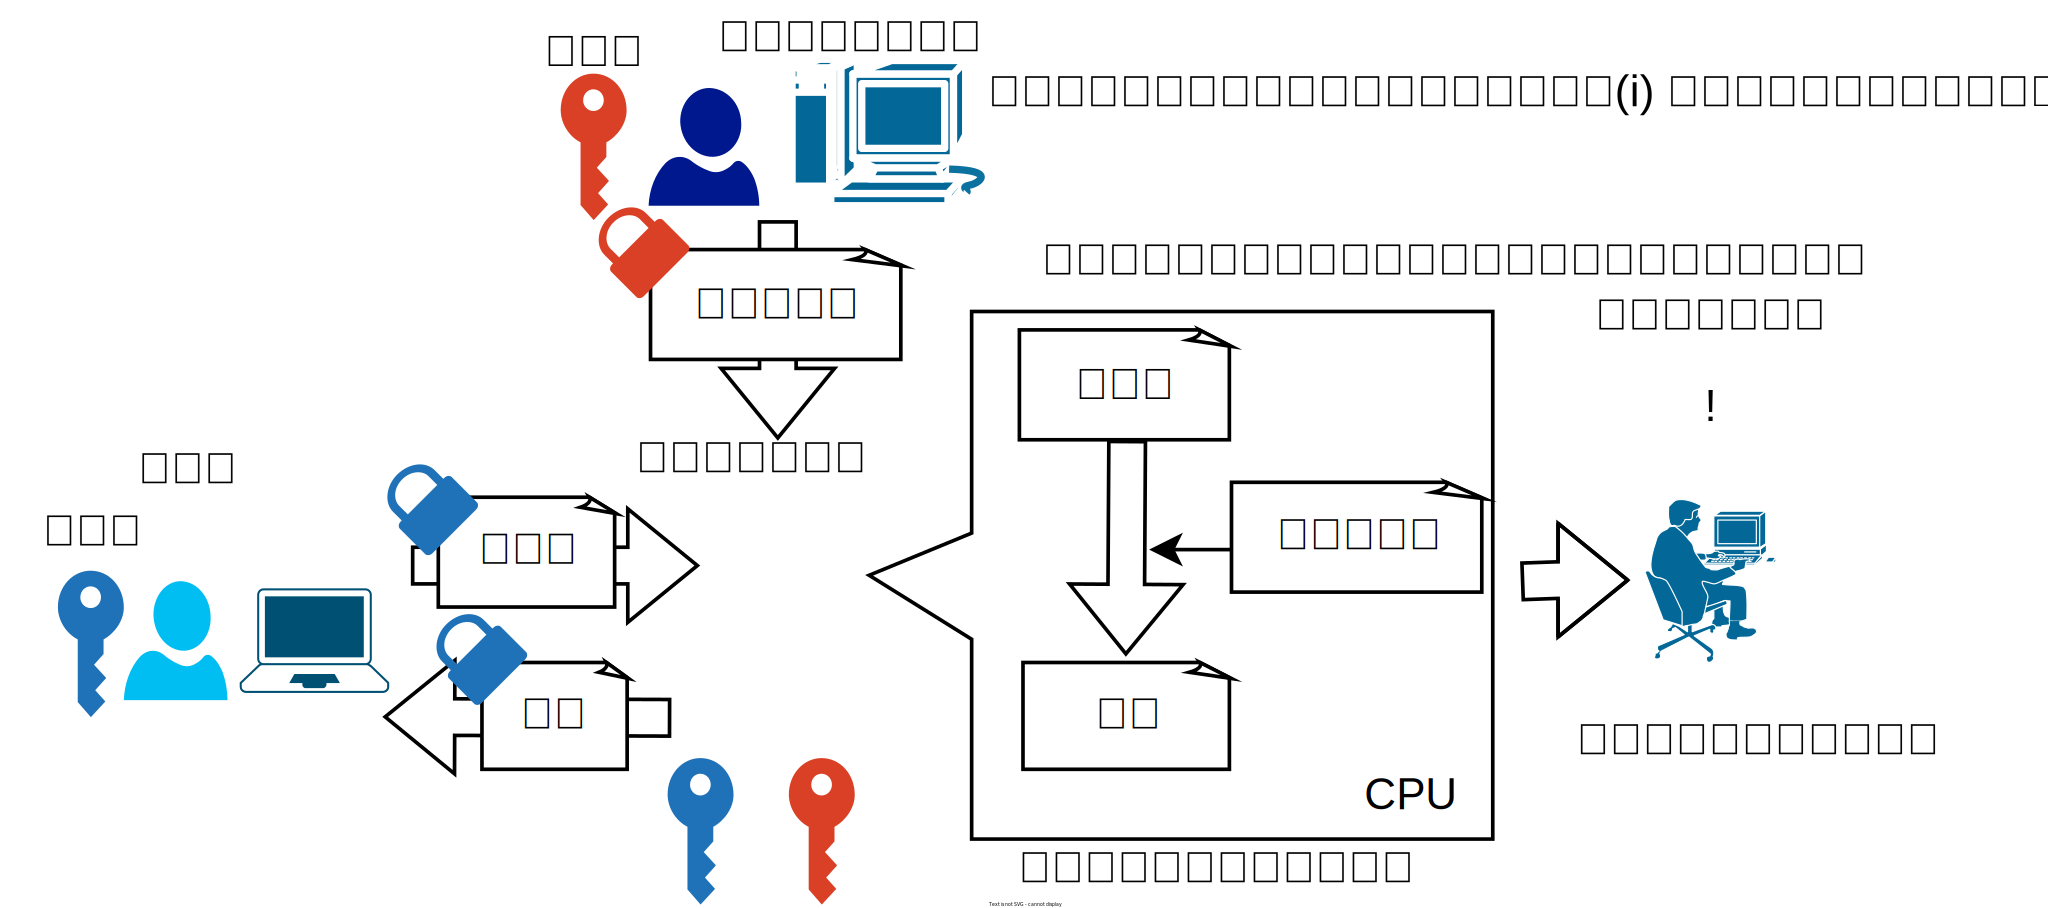
\includegraphics[width=0.8\linewidth]{figures/problem.drawio.pdf}
    \vspace*{-0.5cm}
    \caption{既存のクラウドコンピューティングの問題点}
    \label{fig:problem}
\end{figure}

\noindent[\textbf{課題・分野の状況}]
% 及びー
% 着想に至った経緯にまとめる
% 現状を書く
% ここ短くする
% 現状はいかにまとめる
\begin{enumerate}[label=(\roman*),leftmargin=0.5cm]
\setlength{\parskip}{0cm} % 段落間
\setlength{\itemsep}{0cm} % 項目間
% パラレルにする(利便性の維持を変更するか他を合わせる
    \item \underline{\textbf{データとプログラムがクラウドベンダに見える}}: 図1に示すように、クラウドコンピューティングではサーバ上でデータとプログラムは復号される。準同型暗号を用いれば暗号化したまま計算を行えるが、webサービスのようにプログラム提供者とデータ提供者が分かれる場合、計算量が鍵の本数の2乗に比例する~\ref{paper:mktfhe}ため、計算量が多く現実的でないという問題がある。\label{prob:maliciousvender}
    \item  \underline{\textbf{利便性が損なわれる}}: 申請者の過去の研究~\ref{paper:vsp}では暗号化したままC言語を実行可能にした。しかし、2パーティまでしか対応できず、結果の検証もできない。それに加え、利便性の面でも独自ISAを採用したためにコンパイラも独自で、他の言語のサポートに多大な労力を要する。\label{prob:usability}
    \item  \underline{\textbf{結果がプログラムの出力だと保証できない}}: \amikake{\textbf{Verifiable Computation(VC)}}を用いれば結果がプログラムの実行結果であるかを検証できる。しかし、適用された準同型暗号が限られている~\ref{paper:boostVC}か、実装が存在しない~\ref{paper:nivc}。\label{prob:verifiability}
\end{enumerate}

\noindent[\textbf{着想に至った経緯}]
% 自身の前の研究を欠陥を指摘する感じに

申請者が過去に行った研究~\ref{paper:vsp}では、データ提供者とプログラム提供者が同一である2パーティの場合にプログラムとデータの同時に保護することを可能にした。
しかし、2パーティとして扱えるアプリケーションは限られている。
また、過去の研究のセキュリティの評価を行ううちに、偽の結果を返せることが秘密鍵の流出につながるという脆弱性がある。
そのため、3パーティへの拡張と結果の検証を同時に達成しつつ、過去の研究で重要視していた利便性を維持するものとして本研究計画を着想した。

%end 本研究の着想に至った経緯など ====================

% p01_background_01.tex
\KLEndSubject{F}


